\chapter{Prototipado del algoritmo en software}

\section{Trascurso del algoritmo}
Como se ha explicado anteriormente el algoritmo realizará una recopilación de datos, para obtener 
la señal original del electrocardiograma de cada paciente y asi hacer un filtrado de dicha señal para eliminar
 el ruido y centrarla, seguidamente se realizara la deteccion de picos con algunos metodos como establecer 
 el cutoff dinámico y por último detectar las arritmias y comparar las anotaciones de la señal original con las generadas.
 Véase
  \Cref{fig:esquemaGeneral}.

\begin{figure}[h!]
    \centering
    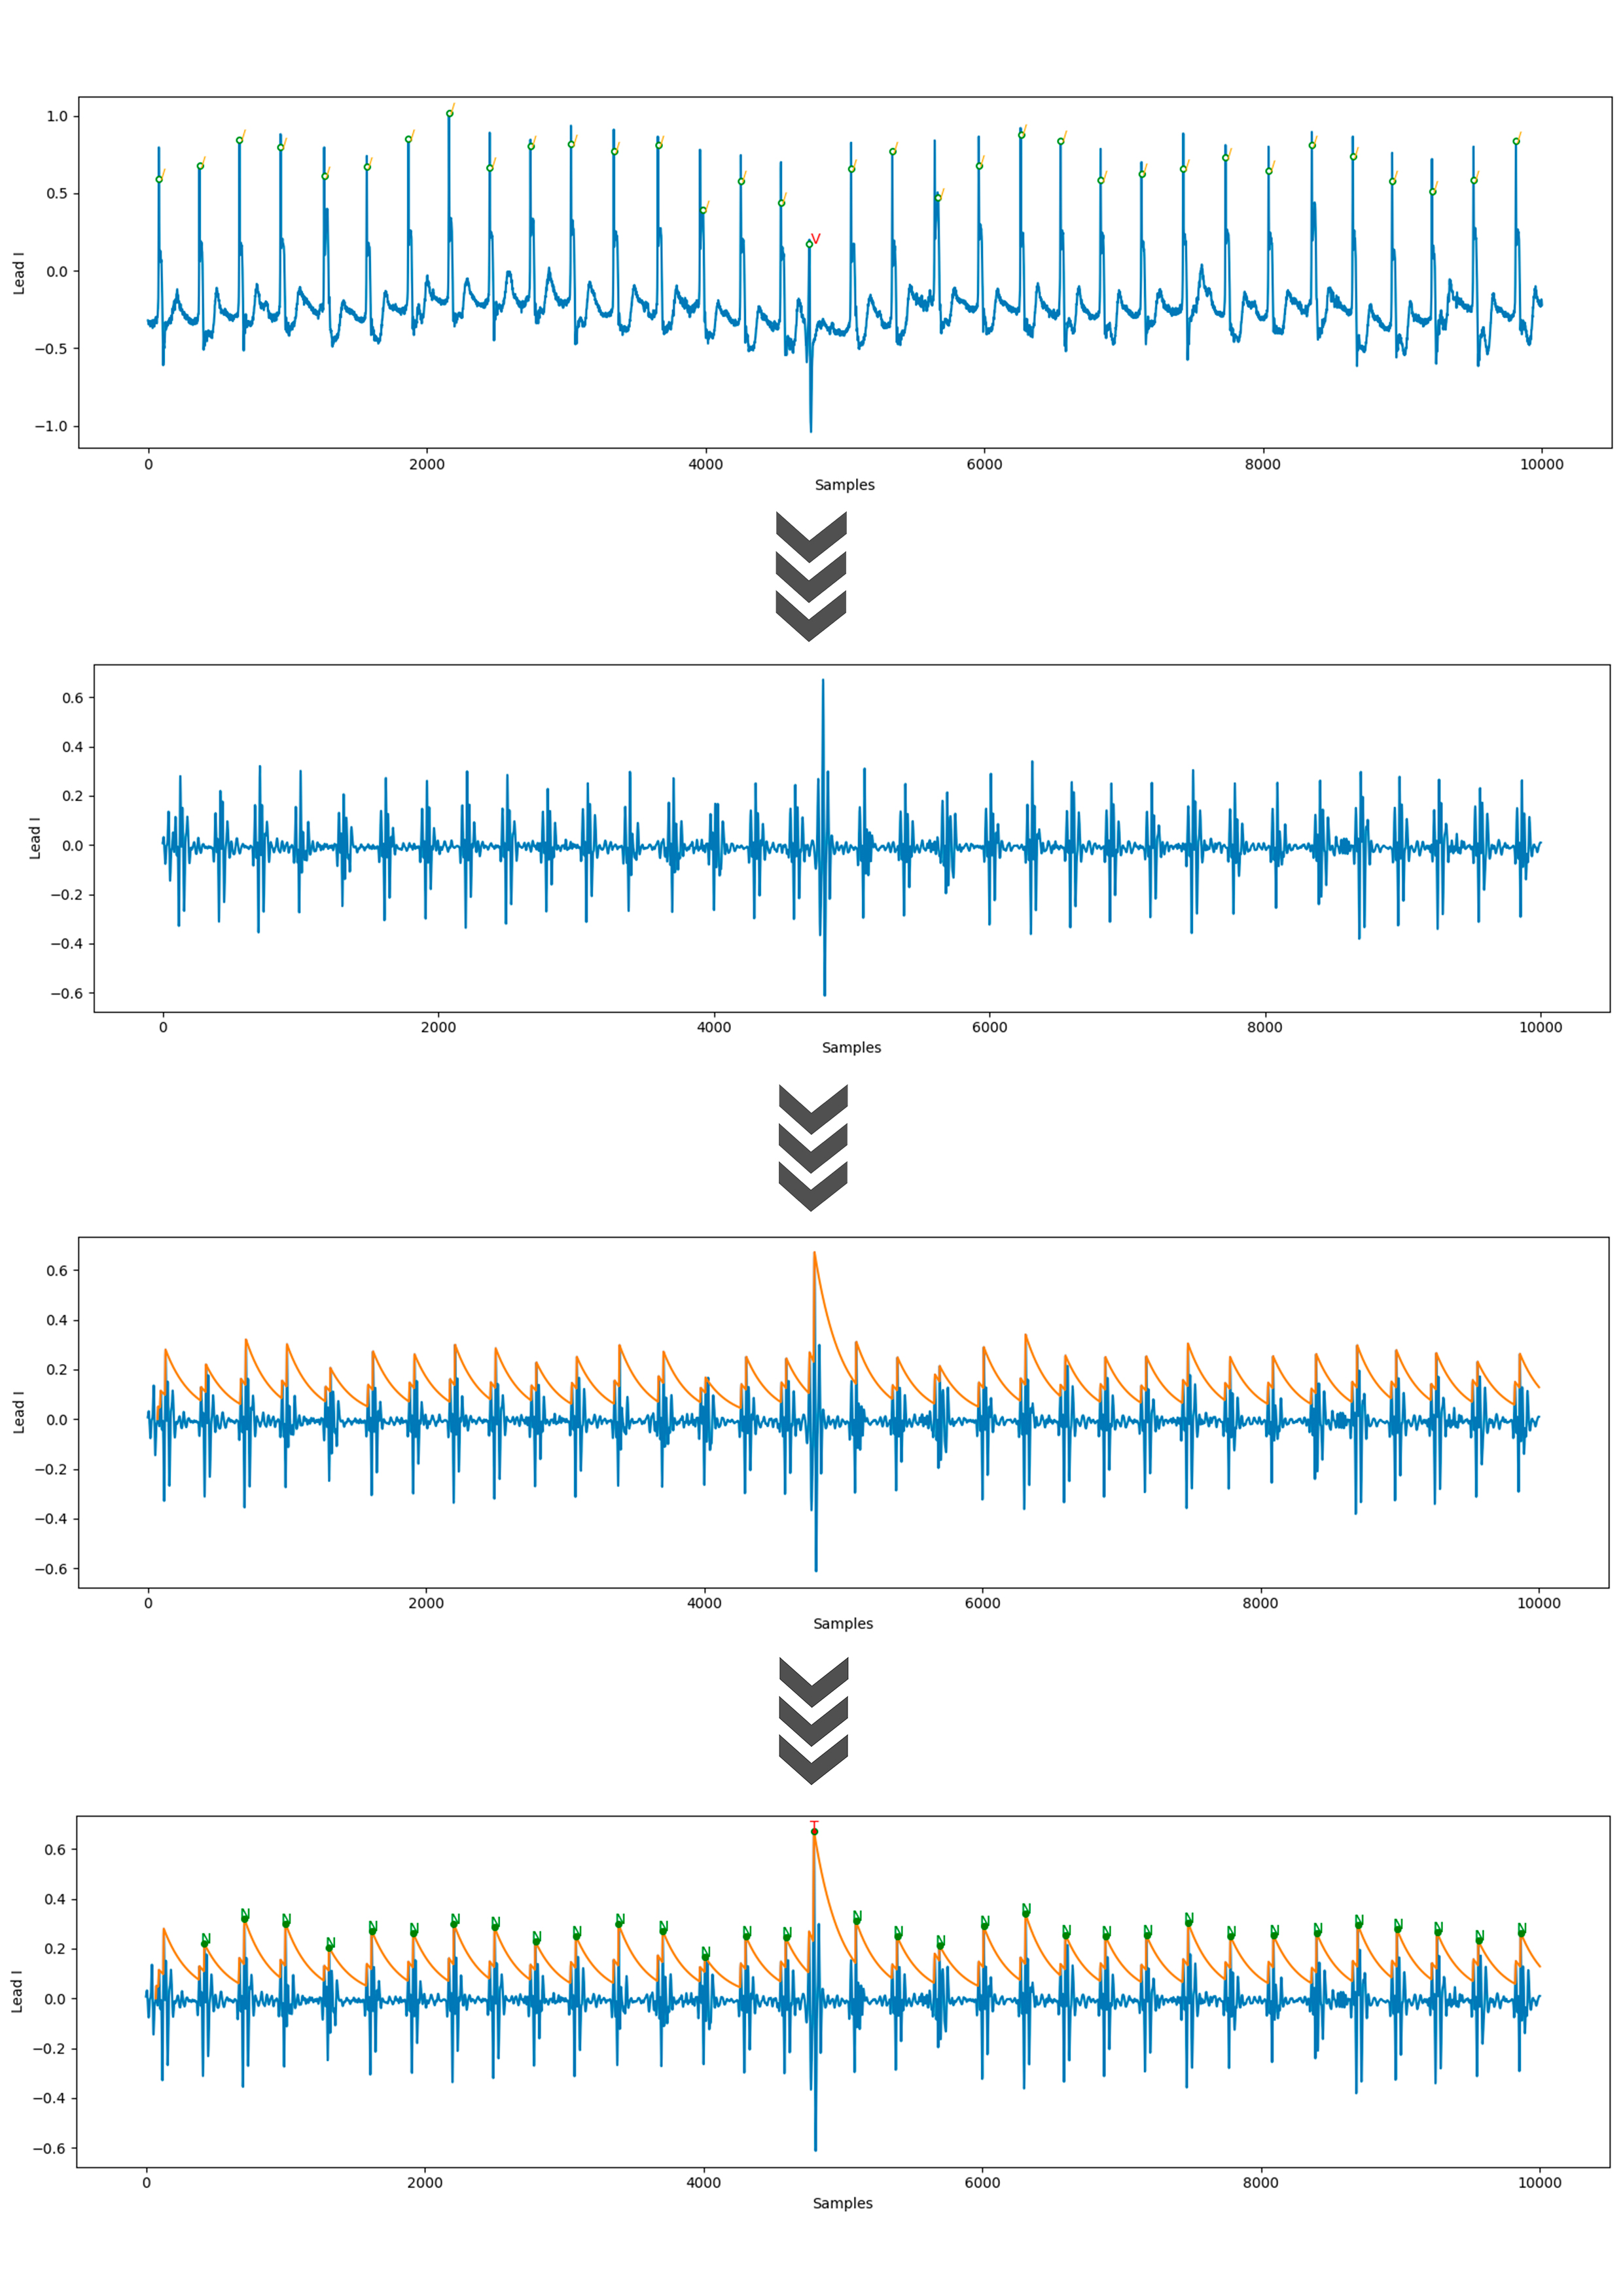
\includegraphics[width=0.7\textwidth]{./Images/img_algoritmo/esquemaGeneral.jpg}
    \caption[Representación del trascurso del prototipo]{Representación del trascurso del algoritmo durante las distintas etapas de su desarrollo}
    \label{fig:esquemaGeneral}
\end{figure}

\section{Recopilación de los datos}
Para la recopilación de los datos se utilizará la librería wfdb que se encarga de proporcionar
funciones para leer y escribir archivos de diferentes formatos que contienen señales biomédicas,
como archivos de registro de señales (por ejemplo, formato .dat), archivos de anotaciones
(por ejemplo, formato .atr) y archivos de cabecera (por ejemplo, formato .hea).

Los pacientes vienen identificados por un identificador (por ejemplo, 101) y hay 3 ficheros por paciente, 
con extensiones .dat, .atr y .hea

Se descarga la base de datos con la función de la librería de wfdb, dldatabase que recoge 
la señal del paciente y las anotaciones de los cardiólogos sobre cada pico QRS.


\lstset{language=python, breaklines=true, basicstyle=\footnotesize}
\begin{lstlisting}[frame=single]
#download the database if not available
if os.path.isdir("mitdb"):
	print('You already have the data.')
else:
	wfdb.dl_database('mitdb', 'mitdb')
\end{lstlisting}

Los pacientes de la base de datos se han hecho una prueba de 30 mins lo que en la señal 
equivale a 650000 samples.

\lstset{language=python, breaklines=true, basicstyle=\footnotesize}
\begin{lstlisting}[frame=single]
sampfrom = 0
sampto = 650000
record = wfdb.rdsamp('mitdb/102', sampfrom=sampfrom, sampto=sampto)
annotation = wfdb.rdann('mitdb/102', 'atr', sampfrom=sampfrom, sampto=sampto)
\end{lstlisting}

Por último, para visualizar esta señal con las anotaciones de los cardiólogos y poder comparar 
con las anotaciones que realiza el algoritmo se usará la librería matplotlib.pyplot.

Con esto se mostrará la señal original con las anotaciones y la señal filtrada con las anotaciones
del algoritmo como en \Cref{fig:102filtradoysinfiltrar}

\section{Filtrado de la señal original}
Este filtrado es llevado a cabo por el filtrado IIR.

El filtrado IIR, que significa \textit{Infinite Impulse Response} (respuesta infinita al impulso),
es un tipo de filtro utilizado en el procesamiento de señales digitales y analógicas.

La fórmula que se utilizará para el filtrado es la siguiente:

\[ Y[i] = \sum_{k=0}^{N_x -1} b_k \cdot x[i-k] \]

Siendo b son los coeficientes del filtrado y x los valores de la señal original a filtrar.

Los coeficientes se almacenan en una lista de 99 valores en punto flotante simétricos que se iteran de forma 
circular, con lo que después de ejecutar el último valor vuelve de nuevo al primero.  

Para el filtrado se usa la función lfilter de la librería scipy.signal

\lstset{language=python, breaklines=true, basicstyle=\footnotesize}
\begin{lstlisting}[frame=single]
    filtered_signal = lfilter(filter_taps_99_6_28, 1.0, original_signal)
\end{lstlisting}

\section{Detección de picos QRS}

El algoritmo de detección de picos está representado en esta función que 
recibe la señal filtrada e intenta detectar los picos QRS.

Este algoritmo está basado en el que se usa en el documento \cite{desai2021low} 
donde en el 4.1.2 muestran una máquina de estados del proceso que realizan.

\begin{figure}[h!]
    \centering
    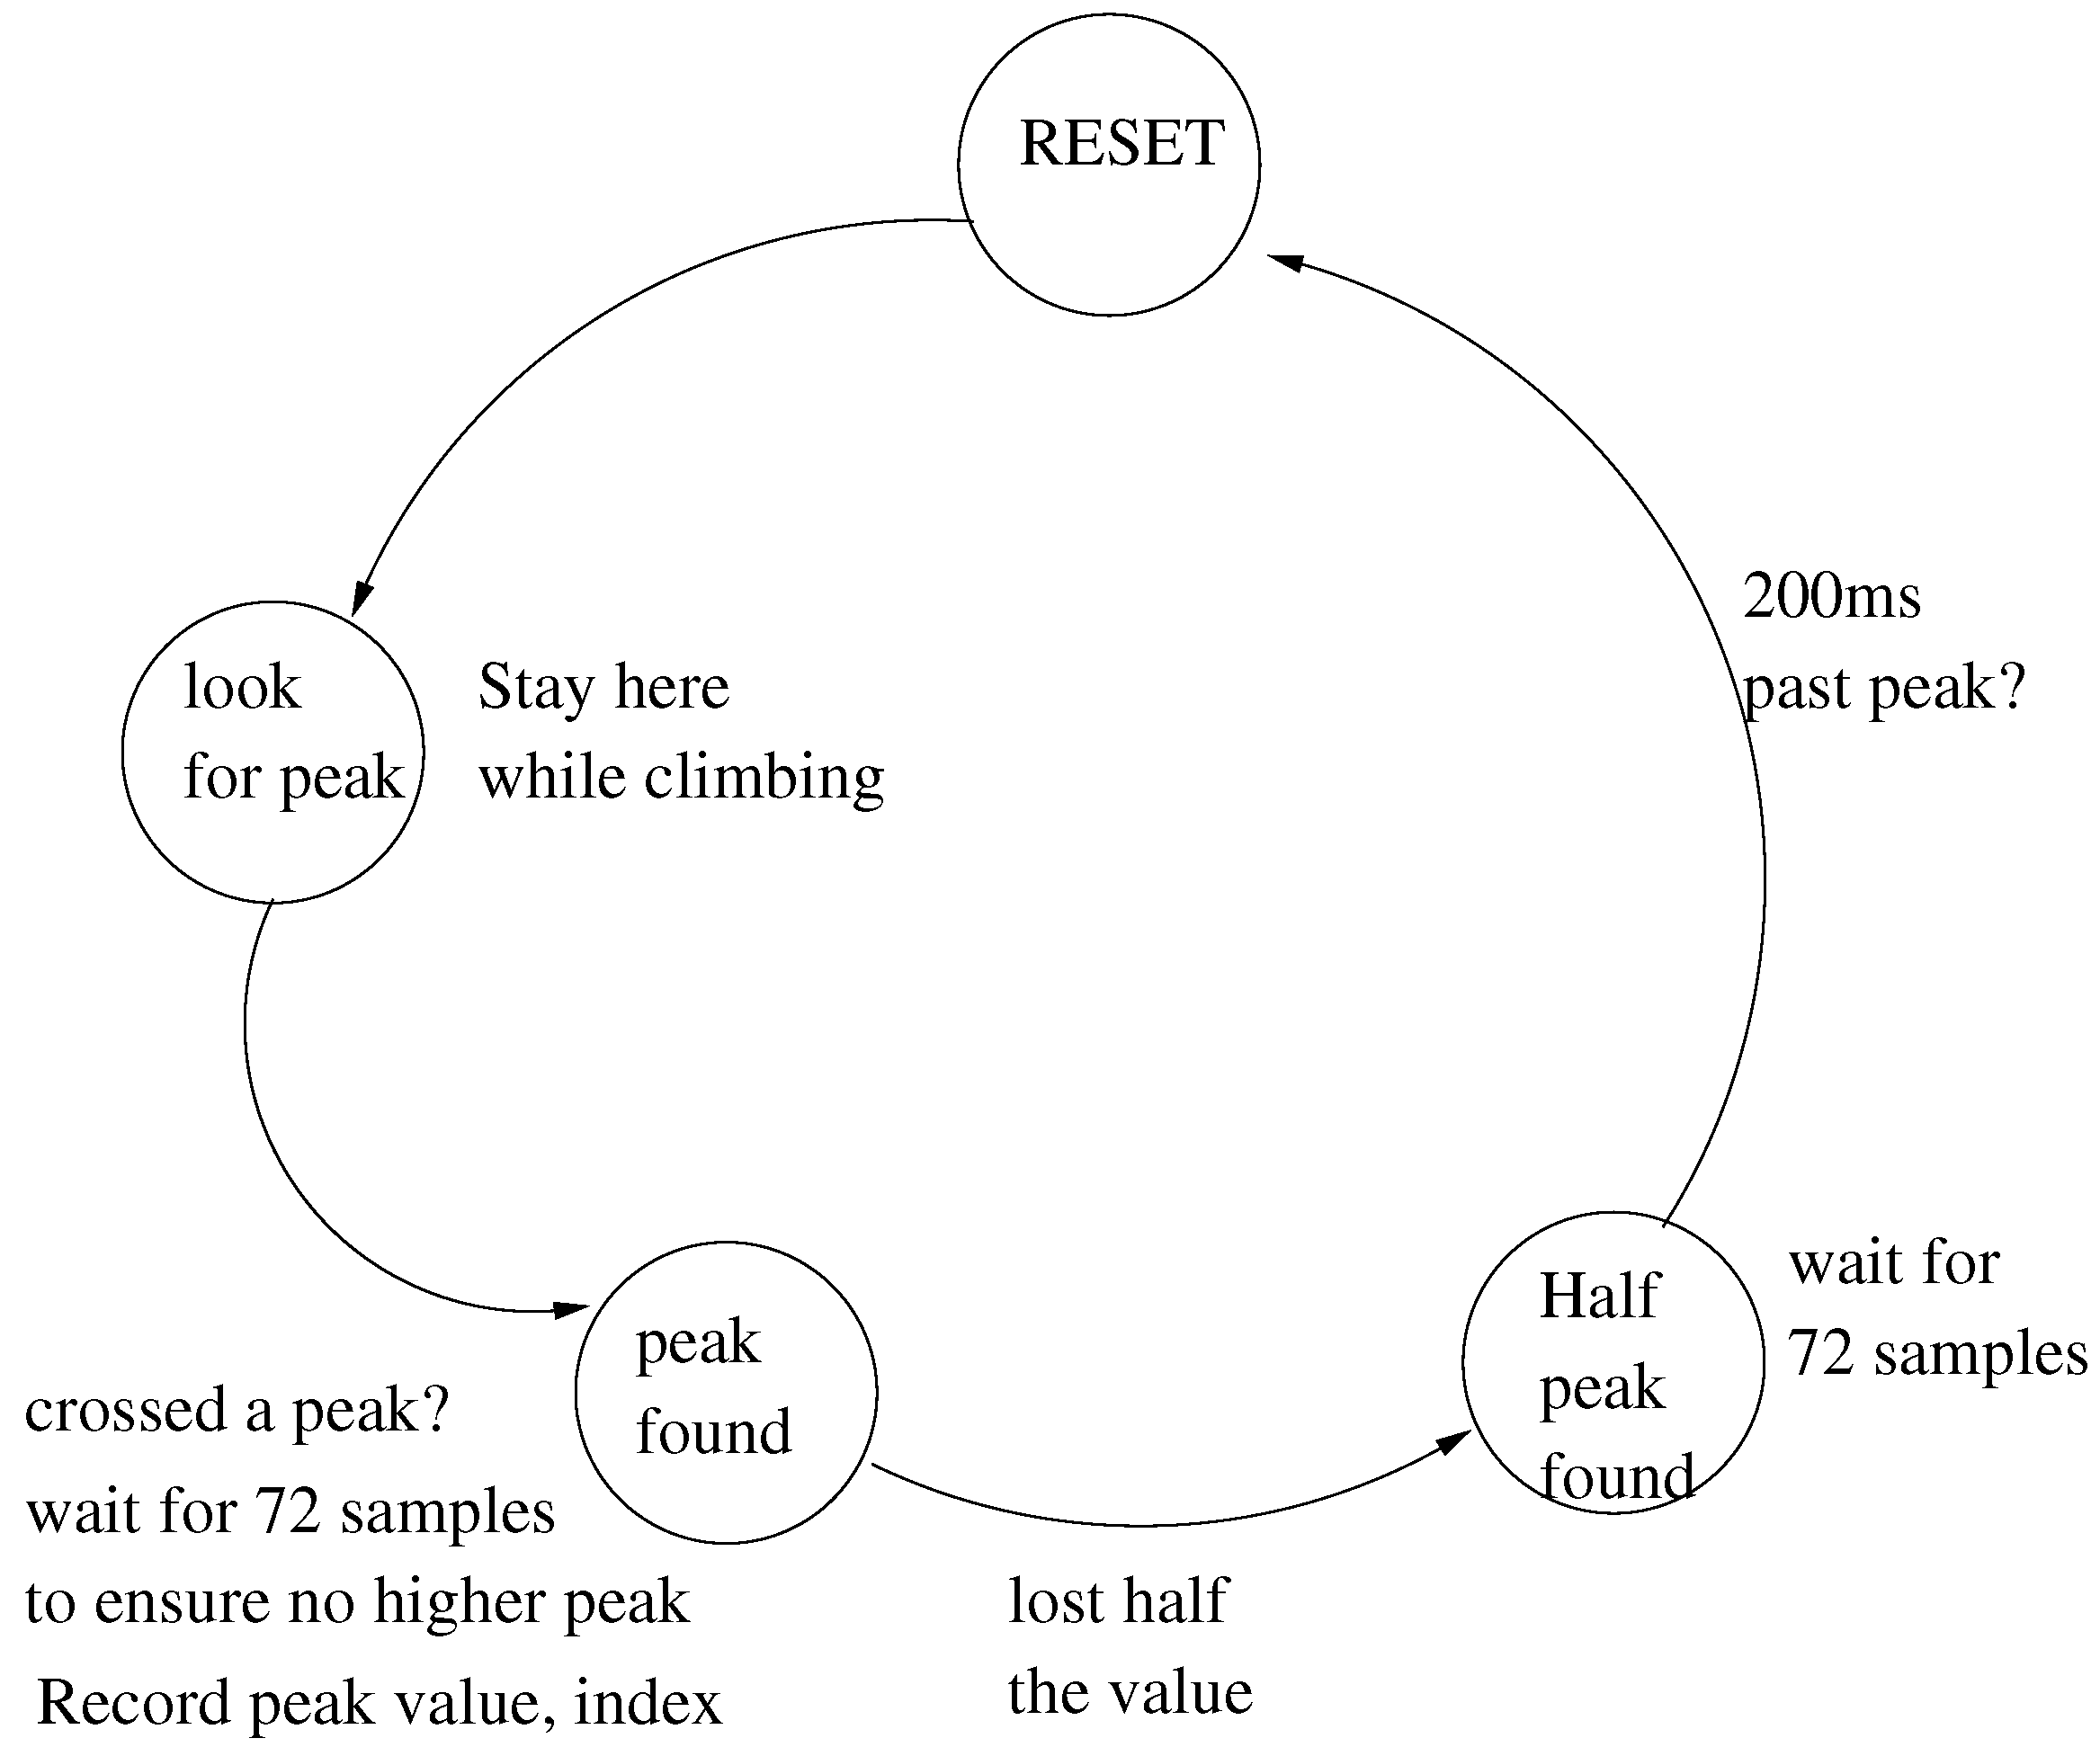
\includegraphics[width=0.6\textwidth]{./Images/img_algoritmo/fsm_mdpi.png}
    \caption{Máquina de estados de algoritmo de detección de picos de estudio de caracterización de señales usando polinomios de Hermite}
    \label{fig:fsm_mpdi}
\end{figure}

El algoritmo realizado es distinto a este, ya que es una versión simplificada de un algoritmo de detección de picos y no llega a ser tan 
funcional por la falta de un cutoff dinámico. Esto se debe a que a veces hay una distancia entre los picos QRS superior a 72 muestras 
por lo que cause que en algunas ocasiones detecte el ruido como un pico QRS, ya que después de las 72 muestras no se ha encontrado una señal.
Es por eso que, en un proyecto en el que se sabe que los picos QRS van a estar a distancias distintas entre si, este algoritmo no sirve y 
hay que modernizarlo.

Aun así, si bien el algoritmo creado es distinto a ese, se replica el tener que esperar a 72 muestras
para asegurarse de que no se encuentra un pico superior y así poder considerarlo como un pico QRS.

Es por ello que definimos la variable \lstinline|samples_around_peak| como 72 para comparar dicha condición.

Para hallar el pico más alto se necesita definir un pico en \lstinline|last_peak| y si se encuentra otro pico se produce

\lstset{language=python, breaklines=true, basicstyle=\footnotesize}
\begin{lstlisting}[frame=single]
last_peak = max(last_peak,signal[i])
\end{lstlisting}

Sin embargo hay un problema y es que cuando se detecte un pico QRS, es decir cuando se haya detectado el pico 
más alto después de haber pasado 72 samples se restauran los valores para empezar a detectar nuevos picos y al
haber ruido el algoritmo podría detectar falsos picos QRS, por ello se debe implementar un \textit{cutoff}.

El \textit{cutoff} es representado como una función descendente que parte de cada pico localizado y mientras no se haya
encontrado ningún pico, el valor de dicha función va decreciendo. La principal función del \textit{cutoff} es evitar que
el algoritmo detecte picos con el ruido y por ello se ha ajustado para que no ocurra el problema anterior y ser capaz de detectar todos los picos QRS.\@

La función del \textit{cutoff} es la siguiente.
    \[cutoff = cutoff - cutoff/(256 - 64)\]


Esta función es llamada cuando no se ha encontrado un nuevo pico y decrementa su valor, cuando se localiza un
nuevo pico, el \textit{cutoff} pasa a tener el valor del pico localizado.

Se han dado los valores (256 - 64) a la formula para que fuese más facil la divison en hardware pero como al final 
se acabo haciendo en un módulo de division en punto flotante cualquier valor es valido para la division aunque debido 
al buen desempeño del valor en el programa se decidio dejar asi.

\lstset{language=python, breaklines=true, basicstyle=\footnotesize}
\begin{lstlisting}[frame=single]
    def extract_peak_indices(signal, total_samples):
        samples_around_peak = total_samples // 2
        last_peak = None
        last_index = None
        peak_indices = []
        cutoff = 0
        for i in range(samples_around_peak-1, len(signal)):
            if last_peak == None:
                last_peak = signal[i]
                last_index = i
                cutoff = calcular_cutoff(cutoff)
            else:
                if signal[i] > last_peak and signal[i] > cutoff:
                    last_peak = signal[i]
                    last_index = i
                    cutoff= signal[i]
                else:
                    if (i - last_index) >= samples_around_peak and last_peak > cutoff:
                        peak_indices.append(last_index)
                        cutoff = calcular_cutoff(cutoff)
                        last_peak = None
                        last_index = None         
                    else:
                        cutoff = calcular_cutoff(cutoff)
            cutoff_plot.append(cutoff)
        ax[1].plot(range(samples_around_peak-1, len(signal)),cutoff_plot)
        return peak_indices
\end{lstlisting}

La salida de dicha función es un buffer de samples que sirven como indices para indicar donde se han encontrado
los picos QRS y asi poder pasar al módulo de detección de arritmias.

\section{Detección de arritmias}

El algoritmo de detección de arritmias se encarga de ver si se ha producido una arritmia según la
distancia entre los picos.

En la detección de arritmias es de vital importancia establecer un límite en la distancia entre los picos
para poder considerar que ha habido una arritmia o no, esta tarea solo se pudo hacer probando con diferentes
rangos y viendo el índice de aciertos producidos en las pruebas a cada paciente de las que se hablara más adelante. 

El algoritmo va almacenando distancias entre los picos QRS (es por ello que en la primera iteración no se almacena nada)
y se declaran varias variables.

\begin{itemize}
    \item last\_distance: se utiliza para almacenar la ultima distancia recogida y asi poder compararla con la distancia 
    actual en calculos posteriores
    \item counter\_buffer: utilizado para tener el valor de la posición del buffer donde se escribe.
    \item counter\_arrythmia: utilizado para indicar si la distancia anterior fue una arritmia.
    \item TNRange: Se utiliza para indicar si hay una distancia más grande de lo normal entre 2 picos QRS producido
    por una arritmia. Es importante tener esta distancia en cuenta, ya que si el ritmo del paciente vuelve a la
    normalidad se compararia la distancia entre el ritmo normal del paciente con el ritmo extendido por la arritmia,
    ya que de no tenerlo en cuenta el algoritmo lo clasificaria como arritmia como se puede ver en la \cref{fig:senial_explicacion_TNRANGE}, por ello se compara con un valor anterior
    que sea el ritmo normal del paciente.
\end{itemize}

\begin{figure}[h!]
    \centering
    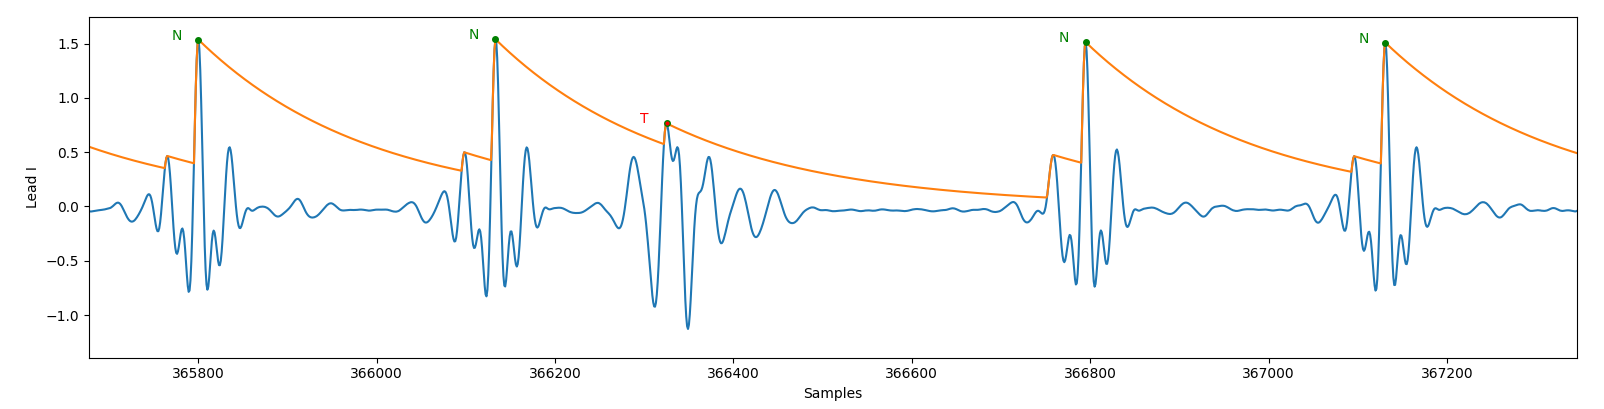
\includegraphics[width=0.9\textwidth]{./Images/img_algoritmo/senial_explicacion_TNRANGE.png}
    \caption{Cuando se detecta una arritmia, a veces, la siguiente distancia es considerablemente más grande de lo normal. Para no detectar falsos positivos, se omite esa distancia}
    \label{fig:senial_explicacion_TNRANGE}
\end{figure}

Por ello si se ha detectado una arritmia, la siguiente distancia se compara con
la tercera última distancia escrita en el buffer que posiblemente sea una distancia causada por un ritmo normal. 
Si no se da el caso, se compara con last\_distance.

la función que compara las distancias devuelve un carácter que va a ser el que se vaya a mostrar en la gráfica, 
si el caracter es "N" significa que se ha detectado un ritmo normal y por tanto solo se muestra. Sin embargo si el 
resultado es "T" significa que la distancia es más corta de lo normal, se detecta la arritmia y se ponen
counter\_arritmia a 1 para saber que la distancia es más corta y TNRange a true para que el algoritmo sepa 
que la distancia que venga después puede ser una ampliada. 

\lstset{language=python, breaklines=true, basicstyle=\footnotesize}
\begin{lstlisting}[frame=single]
    #init the first distance, the first beat doesn't count
    posant = peaks[0]
    last_distance = peaks[1] - peaks[0]

    pos_buffer = [last_distance]
    counterBuffer = 0
    #this var refers to the distance left in between an arrythmia and normal rythm 
    # which tends to be longer. To avoid detection problems we will not compare this distance so the detection can be more precise
    TNRange = False
    counter_arrrythmia = 0
    for pos in peaks[1:]:
        act_distance = pos - posant
        pos_buffer.append(act_distance)
        counterBuffer += 1
    
        if(TNRange==True and counter_arrrythmia == 0):
            sym = get_frecuency_in_char(pos_buffer[counterBuffer - 3],act_distance)
    
            TNRange=False
        else:
            if(TNRange == True):
                counter_arrrythmia -= 1
            sym = get_frecuency_in_char(last_distance,act_distance)
        
    
        if(sym == "N"):
            ax[1].plot(pos, filtered_signal[pos], 'go', markersize=4, markerfacecolor='green')
            ax[1].text(pos-30, filtered_signal[pos], sym, color='green')       
        elif(sym == "T"):
            ax[1].plot(pos, filtered_signal[pos], 'go', markersize=4, markerfacecolor='red')
            ax[1].text(pos-30, filtered_signal[pos], sym, color='red')
            TNRange = True
            counter_arrrythmia = 1
        
        posant = pos
        last_distance = act_distance
\end{lstlisting}

La función get\_frecuency\_in\_char() se encarga de calcular las distancias entre el ritmo actual y un ritmo normal. 
Para ello recibe como entrada ambas distancias.

Para empezar se calcula el gap que es simplemente la diferencia que tiene el la distancia anterior con la actual.
Acto seguido, se calcula el porcentaje de la diferencia de distancia con la distancia anterior que se sabe que va a ser 
un ritmo normal.

Si ese porcentaje es mayor que el 15\% entonces se considera que la distancia normal es mucho mayor que la actual
y por tanto como la distancia actual entre 2 picos es pequeña, se da por hecho que hay una arritmia.

Nótese que no se le da importancia si el gap da como resultado un número negativo de cualquier tamaño, esto se debe
a que este proyecto solo está pensado para detectar contracciones prematuras del corazón, por ende solo necesitamos 
saber si la distancia actual es menor que la anterior. Además ningún paciente parece padecer ninguna arritmia de otro
tipo.

\lstset{language=python, breaklines=true, basicstyle=\footnotesize}
\begin{lstlisting}[frame=single]
def get_frecuency_in_char(last_distance,act_distance): 

    gap = last_distance - act_distance

    percentaje = (gap / last_distance) * 100

    if(percentaje > 15):
        ret = "T"
    else:
        ret = "N"
    return ret

\end{lstlisting}

\section{Pruebas con el algoritmo}

Se han realizado una serie de pruebas para probar el algoritmo estas se encargan de comprobar si las posiciones donde
se ha detectado un pico QRS coinciden con las posiciones de los picos detectados por los cardiólogos, y además se 
encargan de comparar las anotaciones de los cardiólogos con las generadas por el algoritmo.

Con dichas estadísticas es posible comparar el porcentaje de aciertos, en los que se comprende el número de 
falsos positivos, (referido a los ritmos normales que el algoritmo considera arritmias) y 
falsos negativos (referido a las arritmias que el algoritmo considera un ritmo normal).

Para desarrollar estas pruebas, se crea una clase Pair que contenga por cada iteración de la detección de arritmias, el carácter 
por el algoritmo y la posición del sample en la que se encuentre dicho pico QRS.
\newpage
\lstset{language=python, breaklines=true, basicstyle=\footnotesize}
\begin{lstlisting}[frame=single]
class Pair:
def __init__(self, sym, pos):
    self.sym = sym
    self.pos = pos

def __repr__(self):
    return f"Pair({self.sym}, {self.pos})"

\end{lstlisting}

Dicho objeto se inserta en un buffer para luego poder comparar con las anotaciones de la señal original.

\lstset{language=python, breaklines=true, basicstyle=\footnotesize}
\begin{lstlisting}[frame=single]
if(sym == "N" or sym == "T"):
    pair = Pair(sym,pos)    
    produced_symbols.append(pair)
\end{lstlisting}

Una vez se rellena todo el buffer de Pares, se comprueban 2 cosas.
\begin{enumerate}
	\item Si se ha detectado un pico QRS en la señal filtrada y se
     corresponde con el pico de la señal original situado en un sample de una posición aproximada.
	\item Si en el caso de que se haya detectado el pico, las anotaciones de los cardiólogos coinciden
     con las generadas por el algoritmo
\end{enumerate} 

Para este proyecto, solo se valora si el paciente tiene un ritmo normal o una arritmia, pero las anotaciones
que contiene la señal original pueden simbolizar otros problemas como la entrada del marcapasos o otros problemas con la onda T.
En la clase Annotation de la librería wfdb, vienen explicadas todas las posibles anotaciones que puede haber.
\lstset{language=python, breaklines=true, basicstyle=\footnotesize}
\begin{lstlisting}[frame=single]
    ann_labels = [
        AnnotationLabel(0, " ", 'NOTANN', 'Not an actual annotation'),
        AnnotationLabel(1, "N", 'NORMAL', 'Normal beat'),
        AnnotationLabel(2, "L", 'LBBB', 'Left bundle branch block beat'),
        AnnotationLabel(3, "R", 'RBBB', 'Right bundle branch block beat'),
        AnnotationLabel(4, "a", 'ABERR', 'Aberrated atrial premature beat'),
        AnnotationLabel(5, "V", 'PVC', 'Premature ventricular contraction'),
        AnnotationLabel(6, "F", 'FUSION', 'Fusion of ventricular and normal beat'),
        AnnotationLabel(7, "J", 'NPC', 'Nodal (junctional) premature beat'),
        AnnotationLabel(8, "A", 'APC', 'Atrial premature contraction'),
        ...
        AnnotationLabel(12, "/", 'PACE', 'Paced beat'),
        AnnotationLabel(13, "Q", 'UNKNOWN', 'Unclassifiable beat'),
        AnnotationLabel(14, "~", 'NOISE', 'Signal quality change'),
        AnnotationLabel(16, "|", 'ARFCT',  'Isolated QRS-like artifact'),
        ...
        AnnotationLabel(38, "f", 'PFUS',  'Fusion of paced and normal beat'),
        ...
    ]
\end{lstlisting}

Por ello en este proyecto solo se prestará atención a la anotación A y a la anotación V que simbolizan 
las contracciones prematuras de la aurícula y el ventrículo, las demás anotaciones sobre el pico QRS serán 
consideradas como ritmos normales.

Para ver donde se pueden producir posibles errores y el tipo de estos se ha creado un buffer donde en 
cada iteración se hace push de un \textit{string} con el resultado de la señal filtrada y original.

Si por otro lado, el pico no se ha detectado donde tendría que haber un pico QRS puesto en la señal original, 
se pone doble guion para simbolizarlo.

Como se mencionó anteriormente la detección de picos sobre a señal filtrada es aproximado, por lo que se cuenta
si se ha detectado un pico 50 \textit{samples} antes del pico de la señal original y 50 picos después. El número de aproximación 
es moderadamente más amplio para evitar problemas con las posibles imprecisiones del filtrado.  

Otra prueba que se realiza es un conteo de las anotaciones correctas en total, las anotaciones incorrectas en total, las anotaciones
correctas solo de los picos detectados como arritmia, las incorrectas de ese mismo tipo, y los picos no registrados. 
Como se ve en la figura \Cref{fig:estadisticas_algoritmos_1}.

\begin{figure}[h!]
	\centering
    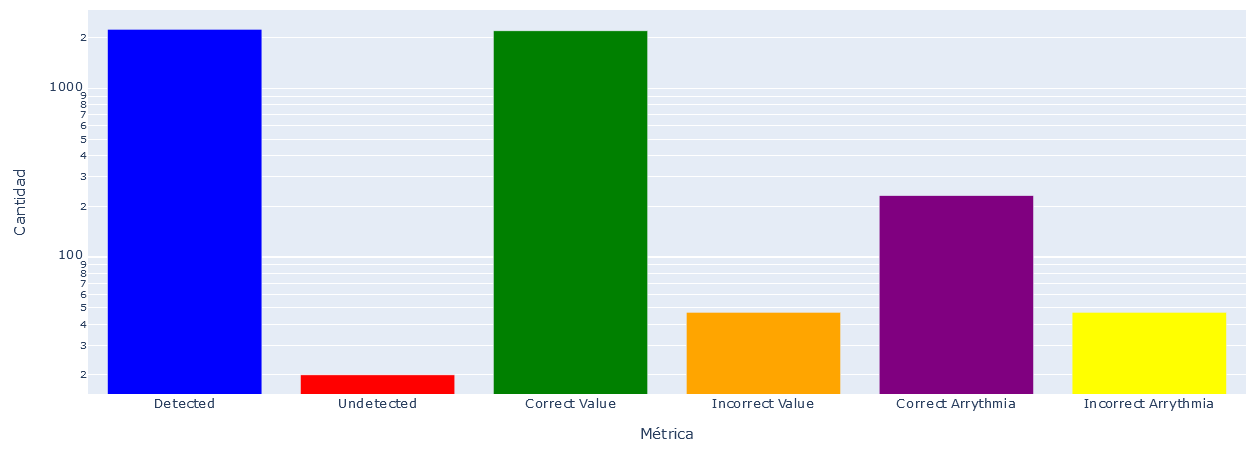
\includegraphics[width=0.9\textwidth]{./Images/img_algoritmo/estadisticas_arritmias_1.png}
    \caption{Métricas de detección de arritmias}
    \label{fig:estadisticas_algoritmos_1}
\end{figure} 

Con el conteo de las anotaciones se pueden sacar varias conclusiones aparte de las dichas 
anteriormente como los picos totales que tiene la señal original, el porcentaje de picos 
detectados, el porcentaje de picos no detectados, el porcentaje de arritmias detectadas 
correctamente, el porcentaje de falsos positivos o falsos negativos, y el porcentaje de éxito de detección de 
arritmias según todas las arritmias contando falsos positivos y negativos. Esto esta representado en la figura \Cref{fig:estadisticas_algoritmos_2}.

\begin{figure}[h!]
	\centering
    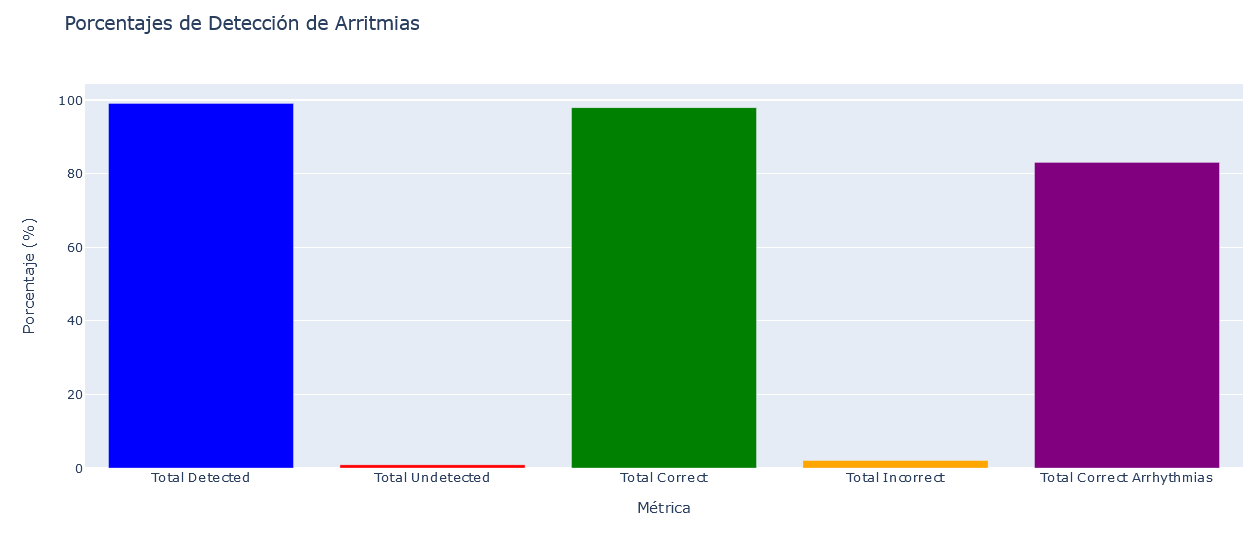
\includegraphics[width=0.9\textwidth]{./Images/img_algoritmo/estadisticas_arritmias_2.png}
    \caption{Porcentajes de detección de arritmias}
    \label{fig:estadisticas_algoritmos_2}
\end{figure} 


Las pruebas que se han realizado se aplican solo para un paciente, pero es posible aplicar estas pruebas a todos los pacientes.
Para ello se ha creado un nuevo fichero de \textit{python} que se encarga de realizar la misma prueba para los pacientes cuyo id está
almacenado en un buffer.

Este programa tiene 2 modos, uno procesa un paciente individualmente y el otro itera una lista con identificadores de los pacientes para procesarlos a todos. La
lógica del algoritmo visto anteriormente está contenida en una nueva función llamada calculations().


Las pruebas que se realizan para este algoritmo son iguales que en el fichero anterior, pero también
se han realizado las siguientes estadísticas.

\begin{enumerate}
	\item La media de los picos detectados de cada paciente.
	\item La media de las arritmias correctas detectadas en cada paciente.
\end{enumerate} 